\documentclass[a4paper, 12pt]{extarticle}
\usepackage{cmap}
\usepackage{amssymb}
\usepackage{amsmath}
\usepackage{graphicx}
\usepackage{amsthm}
\usepackage{upgreek}
\usepackage{listings}
\usepackage{setspace}
\numberwithin{equation}{section}
\usepackage[T2A]{fontenc}
\usepackage[utf8]{inputenc}
\usepackage[normalem]{ulem}
\usepackage{mathtext} % русские буквы в формулах
\usepackage[left=3cm,right=1.5cm,top=2cm,bottom=2cm]{geometry}
\usepackage{linegoal}
\usepackage[english,russian]{babel}
\usepackage[unicode]{hyperref}
\usepackage{pythonhighlight}
\newcommand\Norm[1]{\left\| #1 \right\|}
\newcommand{\dif}{\mathrm{d}}
\newcommand{\Rm}{\mathbb{R}}
\newcommand{\Cm}{\mathbb{C}}
\newcommand{\Z}{\mathbb{Z}}
\newcommand{\I}{\mathbb{I}}
\newcommand{\N}{\mathbb{N}}
\newcommand{\rank}{\operatorname{rank}}
\newcommand{\Ra}{\Rightarrow}
\newcommand{\ra}{\rightarrow}
\newcommand{\FI}{\Phi}
\newcommand{\Sp}{\text{Sp}}
\renewcommand{\leq}{\leqslant}
\renewcommand{\geq}{\geqslant}
\renewcommand{\beta}{\upbeta}
\renewcommand{\gamma}{\upgamma}
\renewcommand{\delta}{\updelta}
\renewcommand{\varphi}{\upvarphi}
\renewcommand{\tau}{\uptau}
\renewcommand{\sigma}{\upsigma}
\renewcommand{\lambda}{\uplambda}
\renewcommand{\psi}{\uppsi}
\renewcommand{\mu}{\upmu}
\renewcommand{\omega}{\upomega}
\renewcommand{\d}{\operatorname{d}}
\renewcommand{\xi}{\upxi}
\renewcommand{\epsilon}{\upvarepsilon}
\newtheorem*{theorem}{Теорема}
\newtheorem*{cor}{Следствие}
\newtheorem*{lem}{Лемма}
\usepackage{stackengine}

% Переоформление некоторых стандартных названий


\begin{document}
	\def\contentsname{ОГЛАВЛЕНИЕ}
	
	% Оформление титульного листа
	\begin{titlepage}
		\begin{center}
			\textsc{МИНИСТЕРСТВО ОБРАЗОВАНИЯ РЕСПУБЛИКИ БЕЛАРУСЬ БЕЛОРУССКИЙ ГОСУДАРСТВЕННЫЙ УНИВЕРСИТЕТ
				\\[5mm]
				ФАКУЛЬТЕТ ПРИКЛАДНОЙ МАТЕМАТИКИ И ИНФОРМАТИКИ\\[2mm]
				Кафедра математического моделирования и анализа данных
			}
			
			\vfill
			
			\textbf{Курсовая работа
				\\[3mm]
				«Прогнозирование временных рядов на основе моделей распознавания заболеваний»
				\\[26mm]
			}
		\end{center}
		
		\hfill
		\begin{minipage}{.5\textwidth}
			\begin{flushright}
				Гут Валерии Александровны\\
				студентки 3 курса 7 группы\\
				специальности «прикладная математика»\\[5mm]
				
				Научный руководитель:\\[2mm] 
				С.В.Лобач\\
				Старший преподаватель\\
				кафедры математического моделирования\\
				и анализа данных ФПМИ
				
			\end{flushright}
		\end{minipage}%
		\vfill
		\begin{center}
			Минск, 2024\ г.
		\end{center}
	\end{titlepage}
	\newpage
	\setcounter{page}{2}
	\begin{center}
		\large{БЕЛОРУССКИЙ ГОСУДАРСТВЕННЫЙ УНИВЕРСИТЕТ}
		\\[2mm]
		Факультет прикладной математики и информатики\\[5mm]
		Кафедра математического моделирования и анализа данных\\[5mm]
		\large{\textbf{ЗАДАНИЕ НА КУРСОВУЮ РАБОТУ\\[20mm]}}
	\end{center}
	Студент \quad \underline{Гут Валерия Александровна\hspace*{\linegoal}}\\[2mm]
	1. Тема \hspace{3mm} Прогнозирование временных рядов на основе моделей \\
	\hspace*{22mm}\underline{распознавания заболеваний\hspace*{\linegoal}}\\[2mm]
	\underline{2. Срок представления курсовой работы к защите  \quad \quad                  17.05.2024 г.\hspace*{\linegoal}}\\[2mm]
	3. Исходные данные для научного исследования\\[2mm]
	3.1 Statistical forecasting of the dynamics of epidemiological indicators for COVID-19 incidence in the Republic of Belarus / Yu. S. Kharin, V. A. Valoshka, O. V. Dernakova, V. I. Malugin, A. Yu. Kharin// Journal of the Belarusian\\
	\underline{State University. Mathematics and Informatics. - 2020. - № 3. - С. 36-50\hspace*{\linegoal}}\\[2mm]
	3.2 Methods of intellectual data analysis in COVID-19 research / O. V. Senko, A. V. Kuznetsova, E. M. Voronin L. R. Borisova, I. L. Kirilyuk // Journal of the Belarusian State University. Mathematics and Informatics. – 2022.\\
	\underline{  – № 1. – С. 83-96.\hspace*{\linegoal}} \\[2mm]
	3.3 Детерминированные и стохастические модели распространения инфекции и тестирование в изолированном контингенте/ Чигарев, А. В.,Журавков, М. А.,Чигарев, В. А.// Журнал Белорусского государственного университета. Математика.\\
	\underline{Информатика - 2021. - № 3. - С. 57-67\hspace*{\linegoal}}\\[2mm]
	3.4 Lazzizzera, I. (2021) An Analytic Approximate Solution of the SIR Model. \\
	\underline{Applied Mathematics, 12, 58-73\hspace*{\linegoal}}\\[2mm]
	4. Содержание курсовой работы\\[2mm]
	4.1 \underline{Рассмотрение различных математических моделей по распознаванию  заболеваний\hspace*{\linegoal}}\\[2mm]
	4.2 Получение основного дифференциального уравнения базовой модели SIR, получение приблизительных аналитического и численного решений. Рандомизация базовой \\ \underline{модели SIR.\hspace*{\linegoal}}\\[2mm]
	4.3 \underline{Подготовить отчет по курсовой работе.\hspace*{\linegoal}}\\[2mm]
	\vfill
	\noindent Руководитель курсовой работы \stackunder{\underline{\hspace*{6cm}Лобач С.В.\hspace*{\linegoal}}}{\textit{подпись, дата\hspace*{2cm}фамилия, инициалы}}\\[2mm]
	Задание принял к выполнению \hspace*{4mm} \stackunder{\underline{\hspace*{6.9cm} Гут В. А. \hspace*{\linegoal}}}{\textit{подпись, дата\hspace*{2cm}фамилия, инициалы}}\\[2mm]
	\newpage
	% Содержание
	\tableofcontents
	\newpage
	\section*{ВВЕДЕНИЕ}\addcontentsline{toc}{section}{ВВЕДЕНИЕ}
	Как показала практика COVID-19, широкое применение современных средств идентификации, диагностики и мониторинга не дает гарантии получения адекватной информации о состоянии индивидуумов в популяции. При моделировании реальных эпидемических процессов на начальных стадиях целесообразно использовать методы эвристического моделирования, а затем уточнять модель с помощью методов математического моделирования, используя стохастические, неопределенно-нечеткие
	методы, позволяющие учитывать то, что протекание, принятие решений, и управление происходит в системах с неполной информацией.
	Для разработки более реалистичных моделей необходим учет пространственной кинетики, что, в свою очередь, требует использования моделей систем с распределенными параметрами (например, моделей механики сплошных сред). Очевидно, что реалистичные модели эпидемий и борьбы с ними должны включать модели экономические, социодинамики. Задачи прогнозирования эпидемий и их развития окажутся не менее сложны, чем задачи прогнозирования изменения климата, прогноза погоды, предсказания землетрясений.
	
	SIR (Susceptible Infections Recovered) модель, описывающая распространение эпидемии, является базовой при применении подходов математического моделирования, так как включает в себя в простейшем варианте основные фазы эпидемии и, в тоже время, допускает их уточнение на основе корректирующих членов в уравнениях, а также добавления в систему  исходных разрешающих уравнений новых уравнений. 
	SIR-модель удобно использовать для модификации детерминированного подхода в вероятностный, так как она учитывает тот факт, что эпидемиологические процессы протекают в условиях наличия неполной информации и погрешностей наблюдения.
	\newpage
	\section{МАТЕМАТИЧЕСКИЕ МОДЕЛИ ЗАБОЛЕВАНИЙ}
	\subsection{Классическая модель SI}
	Данный подход основывается на утверждении: для любого промежутка времени верно, что количество человек, присоединившихся к больным, равно количеству человек, переставших быть здоровыми. Введем следующие обозначения
	\begin{itemize}
		\item $t$ --- независимая переменная, обозначающая время;
		\item $\beta$ -- вероятность заражения здорового человека при контакте с больным;
		\item $S(t)$ -- количество здоровых людей в момент времени $t$; 
		\item $I(t)$ -- количество больных людей в момент времени $t$;
		\item $N = \operatorname{const}$ --- общая численность населения.
	\end{itemize}
	Ввиду этих обозначений имеет место запись $$S(t) + I(t) = N.$$
	Скорость изменения числа здоровых и больных людей с течением времени можно записать, используя аппарат дифференциальных уравнений, в виде следующей системы:
	\begin{eqnarray}
		\left\{ 
		\begin{gathered} 
			\begin{aligned}
				\dfrac{\d S(t)}{\d t} = -\beta\cdot S(t)\cdot I(t),\\
				\dfrac{\d I(t)}{\d t} = \beta\cdot S(t)\cdot I(t).
			\end{aligned}
		\end{gathered} 
		\right.
	\end{eqnarray}
	Используя тот факт, что $S(t) + I(t) = N$, можно переписать эту систему в виде
	\begin{eqnarray}
		\left\{ 
		\begin{gathered} 
			\begin{aligned}
		\dfrac{\d S(t)}{\d t} = -\beta \cdot S(t)\cdot (N - S(t)),\\
		\dfrac{\d I(t)}{\d t} = \beta\cdot (N - I(t))\cdot I(t).
			\end{aligned}
		\end{gathered} 
		\right.
	\end{eqnarray}
	Здесь произведение 
	$$S(t) \cdot (N - S(t)) = I(t)\cdot (N - I(t)) = S(t)\cdot I(t)$$
	равно количеству контактов за единичный промежуток времени в случае, если каждый здоровый контактирует с каждым больным. [3]
	
	В первом уравнении расписано количество ушедших из множества здоровых $S(t)$ (левая часть уравнения) как доля заразившихся при контактах (правая часть уравнения). Во втором уравнении количество новоприбывших в множество больных $I(t)$ (левая часть уравнения) расписывается как доля заразившихся при контактах (правая часть уравнения). Основным недостатком подхода является предположение о том, что больные и здоровые равномерно распределены по пространству. Как следствие, показатель $\beta$ является константой для всех участников социальной сети, и считается, что контакты происходят между всеми парами (больной-здоровый). Также модель предсказывает на уровне численности и не делает никаких предположений о том, кто именно заболевает в следующий момент времени.
	
	
	\subsection{SIR-модель}
	Для анализа и моделирования развития эпидемической ситуации широко используется в практическом использовании модель SIR, основанная на разделении населения на три группы: $S$ -- восприимчивые (Susceptible), $I$ -- инфицированные (Infectious) и $R$ -- имеющие иммунитет (Recovered): $$N = S + I + R,$$ где $N$ -- общая численность населения.
	В этой модели население делится на группы. Ожидается, что каждая группа будет иметь одинаковые характеристики и, получается, что SIR-модель представляет три ветви, сегментированные по модели:
	\begin{itemize}
		\item Susceptible – здоровые люди, которые находятся в группе риска и могут подхватить инфекцию;
		\item Infectious – инфицированные люди; являются переносчиками инфекции;
		\item Recovered – «выбывшие» люди, к которым относятся выздоровевшие люди, приобретшие иммунитет к данной болезни, а также умершие.
	\end{itemize}
	«Восприимчивые» относятся к группе людей, наиболее уязвимых к заболеванию после контакта с инфицированными людьми. На момент заражения они могут уже быть больными или иметь какое-то хроническое заболевание. Группа «инфицированные» представляет уже зараженных инфекцией людей. Они могут передать болезнь группе восприимчивых людей и могут со временем выздороветь. Выздоровевшие пациенты приобретают иммунитет, так как они больше не подвержены этому заболеванию. [5]
	
	Модель SIR задается в общем виде системой обыкновенных дифференциальных уравнений 
	\begin{equation}
		\left\{ 
		\begin{gathered} 
			\begin{aligned}
				\dfrac {\d S(t)}{\d t} &= -\beta \cdot S(t) \cdot I(t),\\
				\dfrac{\d I(t)}{\d t} &= \beta \cdot S(t)\cdot I(t) - \gamma\cdot I(t),\\
				\dfrac{\d R(t)}{\d t} &= \gamma\cdot I(t), 
			\end{aligned}
		\end{gathered} 
		\right.
	\end{equation}
	где $\gamma$ -- интенсивность выздоровления. [3]
	
	Это структура, описывающая, как количество людей в каждой группе изменяется в течении времени. Более подробно вывод этих дифференциальных уравнений описан в главе 2.
	\subsection{Расширения SIR-модели}
	\subsubsection{SIS-модель и SIRD-модель}
	Модель SIS (susceptible-infected-susceptible) основана на предположении, что лица, которые были инфицированы и вылечились, не приобрели
	иммунитет. В этом случае они возвращаются в первую группу восприимчивых. Эта модель задается уравнениями:
	\begin{equation}
		\dfrac{\d S(t)}{\d t} = - \beta\cdot  \dfrac{S(t)\cdot I(t)}{N} + \gamma I(t),
	\end{equation}
	\begin{equation}
		\dfrac{\d I(t)}{\d t} = \beta\cdot  \dfrac{S(t)\cdot I(t)}{N} - \gamma I(t),
	\end{equation}
	В уравнении (6) описывается переход доли лиц, которые были инфицированы, из группы $S(t)$ в группу $I(t)$. Уравнение (7) описывает переход
	доли лиц из группы $I(t)$ снова в $S(t)$, т.е. лиц, которые были инфицированы, вылечились и не получили иммунитет. Данный процесс представлен на Рис. 1.
	\begin{figure}[h]
		\centering
		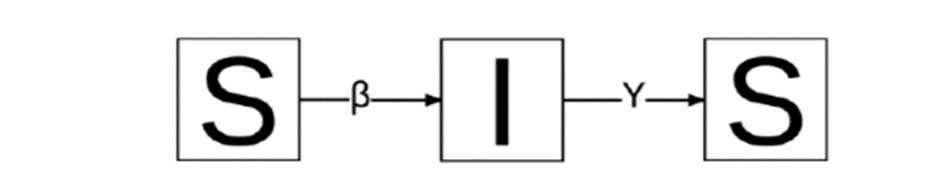
\includegraphics[scale=0.5]{images/img02}
		\caption{Схема перехода индивидов модели SIS.}
		\label{fig:img02}
	\end{figure}
	Для описания некоторых инфекционных заболеваний необходимо рассматривать еще одну группу, описывающую долю умерших индивидов. Как правило, эта группа обозначается буквой $D$ (death). Например, к уже описанной модели SIR добавим группу $D$ и получим модель SIRD. На Рис. 2
	приведена схема новой модели. SIRD модель отличается от классической SIR тем, что инфицированные индивиды могут вылечиться и получить иммунитет с вероятностью $\gamma$ или могут умереть с вероятностью $\mu$. [5]
	\begin{figure}[h]
		\centering
		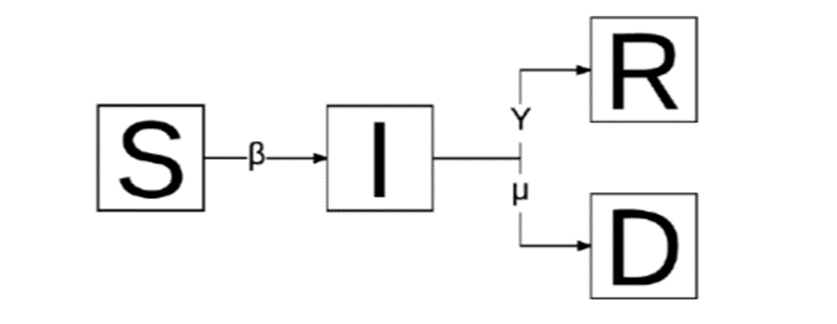
\includegraphics[scale=0.5]{images/img03}
		\caption{Схема перехода индивидов модели SIRD.}
		\label{fig:img03}
	\end{figure}
	
	\subsubsection{Модель SIRS}
	Модель SIRS (Susceptible-Infected-Recovered-Susceptible) является вариацией модели SIR, которая учитывает возможность повторного заражения после выздоровления (потери иммунитета). В модели SIRS существует циклическое движение между состояниями подверженных (S), инфицированных (I) и восстановленных (R). Эта модель задается системой обыкновенных дифференциальных уравнений
	\begin{equation}
		\left\{ 
		\begin{gathered} 
			\begin{aligned}
				\dfrac {\d S(t)}{\d t} &= -\beta \cdot S(t) \cdot I(t) + \lambda \cdot R(t),\\
				\dfrac{\d I(t)}{\d t} &= \beta \cdot S(t)\cdot I(t) - \gamma\cdot I(t),\\
				\dfrac{\d R(t)}{\d t} &= \gamma\cdot I(t) - \lambda \cdot R(t),
			\end{aligned}
		\end{gathered} 
		\right.
	\end{equation}
	где число $\lambda$ определяет вероятность потери иммунитета и перехода из группы $R(t)$ в группу $I(t)$. [2]
	
	Модель SIRS позволяет изучать повторные вспышки болезни в популяции, так как люди, выздоровевшие от инфекции, могут снова стать подверженными и инфицироваться. Это особенно важно для изучения болезней, которые не обеспечивают долгосрочный иммунитет, например, грипп или коронавирусные инфекции.
	
	Решение системы уравнений модели SIRS может быть выполнено с использованием численных методов, таких как метод Эйлера или метод Рунге-Кутты, аналогично модели SIR.
	
	\subsubsection{Модели с учетом смертности и рождаемости особей}
	Для моделирования процессов распространения инфекционных заболеваний в длительные периоды времени необходимо учитывать процессы рождаемости и смертности.
	
	Пусть $\lambda = \operatorname{const} > 0$ и $\mu = \operatorname{const} > 0$ коэффициенты рождаемости и смертности популяции соответственно. Система обыкновенных дифференциальных уравнений для SIR-модели в предположении, что все рожденные являются здоровыми людьми, имеет вид 
	\begin{equation}
		\left\{ 
		\begin{gathered} 
			\begin{aligned}
				\dfrac {\d S(t)}{\d t} &= -\beta \cdot S(t) \cdot I(t) + \lambda\cdot N(t) - \mu\cdot S(t),\\
				\dfrac{\d I(t)}{\d t} &= \beta \cdot S(t)\cdot I(t) - \gamma\cdot I(t) - \mu\cdot I(t),\\
				\dfrac{\d R(t)}{\d t} &= \gamma\cdot I(t) - \mu \cdot R(t),
			\end{aligned}
		\end{gathered} 
		\right.
	\end{equation}
	где $$S(t) + I(t) + R(t) = N(t),$$ причем заметим, что теперь численность популяции $N = N(t)$, то есть она непостоянная (за счет рождаемости и смертности людей). [5]
	
	Складывая все уравнения системы, мы получаем уравнение Мальтуса для численности популяции 
	\begin{equation}
	\dfrac{\d N(t)}{\d t} = (\lambda-\mu) \cdot N(t).
	\end{equation}
	
	Анализируя поведение $I'(0)$, можно определить базовое репродуктивное число. Для отсутствия эпидемии необходимо, чтобы $$\beta S_0 - \gamma - \mu < 0 \quad \text{или}\quad \beta \dfrac{S_0}{\Lambda+\mu} < 1.$$
	Следовательно имеем базовое репродуктивное число для расширенной модели $$R_0 = \beta \cdot \dfrac{S_0}{\Lambda+\mu}.$$ Обратим внимание на то, что коэффициент рождаемости не влияет на пороговый
	эффект. Расширенная SIR-модель с учетом рождаемости и смертности может иметь колеблющиеся решения.
	
	\subsubsection{Модель с учетом инкубационного периода: SEIR-модель}
	SEIR-модель (от англ. Susceptible - Exposed - Infected
	- Removed). Очень часто стандартная модель SIR является слишком простой и
	нереалистичной, так как в ней полагается, что особь является заразной сразу же после инфицирования. В SEIR модели предполагается, что инфекция имеет инкубационный период, в течение которого люди инфицированы, но
	еще не заразны. С учетом нового класса получаем следующую структуру
	популяции:
	$$S + E + I + R = N,$$ где
	\begin{itemize}
		\item $S(t)$ -- это количество не инфицированных людей. Причем скорость изменения количества подверженных зависит от вероятности передачи инфекции, количества инфицированных и количества подверженных, где $\beta$ -- это скорость передачи заболевания;
		\item $E(t)$ -- это число инфицированных, но еще не заразных людей. Причем скорость изменения количества инфицированных, но еще не заразных людей зависит от входящего потока людей, проходящих инкубационный период, а также выходящего потока этих же людей. Параметр $\sigma^{-1}$ представляет собой среднюю продолжительность инкубационного периода;
		\item $I(t)$ -- это количество инфицированных людей. Причем	скорость изменения количества инфицированных зависит от входящего потока инфицированных и выходящего потока инфицированных. Параметр $\gamma$ -- это скорость восстановления;
		\item $R(t)$ -- это группа выздоровевших лиц, а именно людей, которые восстановились.
	\end{itemize}
	Модель SEIR задается в общем виде системой обыкновенных дифференциальных
	\begin{equation}
		\left\{ 
		\begin{gathered} 
			\begin{aligned}
				\dfrac {\d S(t)}{\d t} &= - \beta \cdot I(t)\cdot S(t),\\
				\dfrac {\d E(t)}{\d t} &= \beta \cdot S(t)\cdot I(t) - \sigma\cdot E(t),\\
				\dfrac{\d I(t)}{\d t} &=\sigma \cdot E(t) - \gamma\cdot I(t),\\
				\dfrac{\d R(t)}{\d t} &= \gamma\cdot I(t). 
			\end{aligned}
		\end{gathered} 
		\right.
	\end{equation}
	Также имеет место модель SEIR с учетом смертности и рождаемости особей, которая задается системой обыкновенных дифференциальных уравнений [2]
	\begin{equation}
		\left\{ 
		\begin{gathered} 
			\begin{aligned}
				\dfrac {\d S(t)}{\d t} &= \lambda N(t) - (\beta \cdot I(t) +\mu)\cdot S(t),\\
				\dfrac {\d E(t)}{\d t} &= \beta \cdot S(t)\cdot I(t) - (\mu + \sigma)\cdot E(t),\\
				\dfrac{\d I(t)}{\d t} &=\sigma \cdot E(t) - (\mu + \gamma)\cdot I(t),\\
				\dfrac{\d R(t)}{\d t} &= \gamma\cdot I(t) - \mu \cdot R(t). 
			\end{aligned}
		\end{gathered} 
		\right.
	\end{equation}
	Модель SIER может быть реализована с помощью численных методов, таких как метод Эйлера или метод Рунге-Кутты, для решения системы дифференциальных уравнений. Исходные значения для каждой группы (S, E, I, R) задаются в начальный момент времени, и затем численные методы используются для вычисления значений в каждый последующий момент времени.
	Важно отметить, что модель SIER является упрощенной моделью и не учитывает множество реальных факторов, таких как вакцинация, мутации вируса и изменение поведения людей. Но она предоставляет базовый фреймворк для изучения распространения инфекции и позволяет прогнозировать общую динамику эпидемии.
	
	Дополнительные вариации модели SIER также могут включать дополнительные факторы, такие как иммунизация или введение противоэпидемических мер. Модель SIER и ее вариации широко используются в исследованиях эпидемиологии и планировании общественного здравоохранения. Они позволяют ученым и решающим органам оценить различные стратегии контроля эпидемии, такие как вакцинация, социальное дистанцирование, использование масок и карантинные меры. Такие модели могут помочь прогнозировать будущие тенденции распространения болезни и определить наиболее эффективные меры по сдерживанию инфекции.
	
	\subsubsection{Модель MSIR}
	Модель MSIR (M — «maternally derived immunity») включает класс $M(t)$ (для материнского иммунитета) в начало модели. Модель MSIR описывается следующими дифференциальными уравнениями:
	\begin{equation}
		\left\{ 
		\begin{gathered} 
			\begin{aligned}
				\dfrac {\d M(t)}{\d t} &= \lambda N(t) - \delta\cdot M(t)-\mu\cdot M(t),\\
				\dfrac {\d S(t)}{\d t} &= \delta \cdot M(t) -\beta\cdot S(t)\cdot I(t) - \mu \cdot S(t),\\
				\dfrac{\d I(t)}{\d t} &=\beta\cdot S(t)\cdot I(t) - \gamma \cdot S(t) - \mu \cdot I(t),\\
				\dfrac{\d R(t)}{\d t} &= \gamma\cdot I(t) - \mu \cdot R(t), 
			\end{aligned}
		\end{gathered} 
		\right.
	\end{equation}
	где $S(t) + I(t) + R(t) = N(t).$ [4]
	\subsubsection{Модель MSEIR}
	Модель MSEIR ($M$ -- наделенные иммунитетом от рождения, $S$ -- восприимчивые, $E$ -- контактные, $I$ -- инфицированные, $R$ -- выздоровевшие) -- одна из самых сложных для анализа в силу наличия большого числа независимых параметров. Система уравнений для нее имеет вид:
	\begin{equation}
		\left\{ 
		\begin{gathered} 
			\begin{aligned}
				\dfrac {\d M(t)}{\d t} &= \Lambda(t) - \delta\cdot M(t)-\mu\cdot M(t),\\
				\dfrac {\d S(t)}{\d t} &= \delta \cdot M(t) -\beta\cdot S(t)\cdot I(t) - \mu \cdot S(t),\\
				\dfrac {\d E(t)}{\d t} &= \beta \cdot S(t)\cdot I(t) - (\epsilon + \mu)\cdot E(t),\\
				\dfrac{\d I(t)}{\d t} &=\epsilon \cdot E(t) - (\gamma + \mu)\cdot I(t),\\
				\dfrac{\d R(t)}{\d t} &= \gamma\cdot I(t) - \mu \cdot R(t). 
			\end{aligned}
		\end{gathered} 
		\right.
	\end{equation}
	где $M (t)$ -- численность индивидов с приобретенным внутриутробно иммунитетом. От ранее рассмотренных моделей эта система (13) отличается тем, что учитывает рождение детей, вероятность заражения которых растет со временем по мере утраты ими иммунитета, приобретенного внутриутробно. Эти зависимости описаны в первых двух уравнениях системы (13). [5]
	
	Приобретенный внутриутробно иммунитет $V(t)$ может быть не у всех появившихся на свет детей, но вакцинацией можно охватить сто процентов рожденных младенцев. Введение в математическую модель этого параметра приводит к качественному изменению картины развития эпидемий. Система дифференциальных уравнений для этой модели будет следующей:
	\begin{equation}
		\left\{ 
		\begin{gathered} 
			\begin{aligned}
				\dfrac {\d S(t)}{\d t} &= \mu \cdot N\cdot (1-P) - \mu \cdot S(t) - \beta \dfrac{I(t)}{N}\cdot S(t),\\
				\dfrac{\d I(t)}{\d t} &=\beta \cdot \dfrac{I(t)}{N}\cdot S(t) - (\gamma + \mu)\cdot I(t),\\
				\dfrac{\d V(t)}{\d t} &= \mu \cdot N \cdot P - \mu \cdot V(t). 
			\end{aligned}
		\end{gathered} 
		\right.
	\end{equation}
	где $P$ -- доля привитых младенцев $( 0 < P < 1 )$. Первые два уравнения системы $(14)$ повторяют модель SIR с учетом того, что вероятность заражения привитых детей равна нулю, а значит, вероятность заражения равна вероятности, что ребенок не привит, и, в свою очередь, равна $(1 - P)$. Последнее уравнение системы $(14)$ учитывает смертность от других причин и позволяет рассчитать полную численность популяции.
	\newpage
	\section{БАЗОВАЯ МОДЕЛЬ SIR И ЕЕ РАНДОМИЗАЦИЯ}
	\subsection{Базовая SIR-модель}
	Модель SIR (модель Кермака-Маккедрика сформулированная в 1927 году) -- одна из простейших компартментных моделей, в которых с помощью систем дифференциальных уравнений описывается динамика групп восприимчивых, инфицированных и выздоровевших индивидов. Многие модели являются производными от этой базовой формы. Для того, чтобы ее сформулировать, введем следующие обозначения:
	\begin{itemize}
		\item независимая переменная $t$ -- время;
		\item число $N \in \Rm$ -- постоянная численность популяции;
		\item функция $S(t)$ -- группа членов популяции, которые потенциально могут быть инфицированы (Susceptible);
		\item функция $I(t)$ -- количество инфицированных (Infected);
		\item функция $R(t)$ -- количество выздоровевших, «привитых» и умерших (Recovered).
	\end{itemize}	
	Будем также предполагать, что рождаемость и смертность, не связанная с эпидемией, могут игнорироваться и что инкубационный период тоже ничтожно мал. Тогда мы мы можем смоделировать следующее уравнение для любого момента времени
	\begin{eqnarray}
		S(t) + I(t) + R(t) = N.
	\end{eqnarray}
	Из полученного уравнения (1) следует, что существует три основные группы членов в рассматриваемой
	популяции, численность в каждой из которых переменная, причем изменения
	направлены в одну сторону: $$S \to I \to R.$$
	Ввиду приведенных обозначений и формулируется название модели как SIR-модель. 
	
	\subsubsection{Построение задачи Коши для базовой SIR-модели.}
	Рассмотрим начальный момент времени $t_0$, то есть начало эпидемии в данном случае. Пусть у нас имеется один инфицированный индивидуум из группы $I(t)$ и некоторое количество восприимчивых людей из группы $S(t)$. В результате контактов, данный инфицированный индивидуум заражает какое-то количество восприимчивых, тем самым переводит их из группы $S(t)$ в группу $I(t)$, то есть совершается переход $$S \to I.$$
	Введем новую величину $\beta$ -- интенсивность заражения или же  среднее количество контактов на одного человека во времени. Тогда мы можем считать, что один инфицированный заразил в среднем $\beta$ индивидуумов за единицу времени.
	
	Для дальнейшего описания в уравнении (1), предполагая $N\ne 0$, разделим обе части уравнения на $N$ и получим 
	\begin{eqnarray}
		\dfrac{S(t)}{N} + \dfrac{I(t)}{N} + \dfrac{R(t)}N = 1.
	\end{eqnarray}
	Тогда мы имеем следующие функции:
	\begin{itemize}
		\item $s(t) = \dfrac {S(t)} N$ -- доля подверженных инфицированию индивидуумов;
		\item $i(t) = \dfrac{I(t)} N$ -- доля инфицированных индивидуумов;
		\item $r(t) = \dfrac{R(t)} N$ -- доля выздоровевших, «привитых» и умерших индивидуумов.
	\end{itemize}
	
	Теперь рассмотрим середину эпидемии. Пусть к этому моменту в популяции, кроме двух упомянутых категорий людей, появились переболевшие или выздоровевшие индивидуумы из группы $R(t)$, то есть осуществлялся переход $$I \to R.$$ Рассмотрим конкретного инфицированного и оценим, сколько людей он может заразить. Причем это число уже не равно $\beta$, потому что у нас в популяции есть люди
	невосприимчивые к данной инфекции. Поэтому значение $\beta$ надо уменьшить, а именно умножить на долю всех восприимчивых людей в данный момент времени в популяции $\beta \cdot s(t)$. Таким образом это и есть количество инфицированных людей за единицу времени одним конкретным человеком. 
	
	Общее количество всех инфицированных за единицу времени увеличивается на
	величину $$\beta \cdot s(t) \cdot i(t).$$
	Отметим, что величина $s(t)\cdot i(t)$
	представляет собой плотность контактов между членами групп
	$S(t)$ и $I(t)$.
	
	С другой стороны, изменение величины за единицу времени из физических соображений понимается как скорость, которая определяется как производная этой величины по времени. Тогда мы можем записать введенную  скорость изменения плотности подверженных инфицированию как 
	\begin{eqnarray}
		\dfrac {\d s(t)}{\d t} = -\beta \cdot s(t) \cdot i(t),
	\end{eqnarray}
	причем доля восприимчивых индивидуумов за единицу времени
	уменьшается на данную величину, поэтому спереди ставим знак « $-$ ».
	Реальное же значение количестве всех инфицированных за единицу времени будет несколько отличаться от наших вычислений, оно будет меньше, так как, разные инфицированные могут заразить одного и того же человека, но мы этим пренебрегаем. 
	
	Далее для исследования изменения доли инфицированных людей за единицу времени мы введем еще одну величину $\gamma$ -- интенсивность выздоровления. Она выражает количество людей, которые
	выздоравливают и переходят в группу $R(t)$ за единицу времени. Например, если болезнь длится $D$ дней, и в течение этого
	периода инфицированный индивидуум может заразить еще кого-то, то $$\gamma = \dfrac 1D.$$
	В среднем $\frac 1D$ всех инфицированных переходит в категорию выздоровевших за единицу времени.
	
	Ввиду определенной величины $\gamma$, мы можем теперь оценить скорость изменения доли инфицированных людей за единицу времени как \begin{eqnarray}
		\dfrac{\d i(t)}{\d t} = \beta \cdot s(t)\cdot i(t) - \gamma\cdot i(t).
	\end{eqnarray}
	Отметим, что описанная простейшая модель не содержит демографических
	факторов (рождение, смертность от других причин). Таким образом она пригодна для
	краткосрочного прогноза, когда количество новорожденных и умерших за
	рассматриваемый период сравнительно мало (т.е. $N\approx \operatorname{const}$).
	
	Остается определить скорость изменения доли выздоровевших, «привитых» и умерших за единицу времени. С использованием введенных обозначений мы можем ее запросто определить как  
	\begin{eqnarray}
		\dfrac{\d r(t)}{\d t} = \gamma\cdot i(t).
	\end{eqnarray}
	
	Таким образом, собрав все полученные уравнения (3)-(5), мы получаем систему обыкновенных дифференциальных уравнений
	\begin{equation}
		\left\{ 
		\begin{gathered} 
			\begin{aligned}
				\dfrac {\d s(t)}{\d t} &= -\beta \cdot s(t) \cdot i(t),\\
				\dfrac{\d i(t)}{\d t} &= \beta \cdot s(t)\cdot i(t) - \gamma\cdot i(t),\\
				\dfrac{\d r(t)}{\d t} &= \gamma\cdot i(t). 
			\end{aligned}
		\end{gathered} 
		\right.		
	\end{equation}
	Причем, сложив все уравнения, мы получим 
	\begin{equation}
		\dfrac {\d s(t)}{\d t} + \dfrac {\d i(t)}{\d t} + \dfrac {\d r(t)}{\d t} = 0,
	\end{equation}
	а в силу уравнения (2), имеем 
	\begin{equation}
		s(t) + i(t) + r(t) = 1.
	\end{equation}
	Теперь необходимо поставить задачу для системы уравнений (6). Наложим следующие начальные условия 
	\begin{equation}
		s(t)\Big|_{t=t_0} = s_0 \approx 1,\quad i(t)\Big|_{t=t_0} = i_0 << 1,\quad r(t)\Big|_{t=t_0} = 0,
	\end{equation}
	которые в нашем случае определяют начало эпидемии следующим образом: в начальный момент времени $t_0$ у нас есть некоторая группа $S(t_0)$ восприимчивых индивидуумов, которая стремится к числу $N$ (так как $s_0 = \frac{S(t_0)}N$), и некоторая группа $I(t_0)$ инфицированных индивидуумов (так как $i_0 = \frac{I(t_0)}N$), которая много меньше $N$, а количество выздоровевших индивидуумов равно нулю.
	
	Собрав воедино систему (6) и начальные условия (9) мы получаем задачу Коши, которая является математической моделью распространения эпидемии 
	$$
	\left\{ 
	\begin{gathered} 
		\begin{aligned}
			\dfrac {\d s(t)}{\d t} &= -\beta \cdot s(t) \cdot i(t),\\
			\dfrac{\d i(t)}{\d t} &= \beta \cdot s(t)\cdot i(t) - \gamma\cdot i(t),\\
			\dfrac{\d r(t)}{\d t} &= \gamma\cdot i(t). 
		\end{aligned}
	\end{gathered} 
	\right.
	$$
	$$
	s(t)\Big|_{t=t_0} = s_0,\quad i(t)\Big|_{t=t_0} = i_0,\quad r(t)\Big|_{t=t_0} = 0.
	$$
	\subsubsection{Аналитическое решение задачи Коши для базовой SIR-модели}
	Рассмотрим составленную задачу Коши (6), (9) вместе с уравнением (8)
	$$
	\left\{ 
	\begin{gathered} 
		\begin{aligned}
			\dfrac {\d s(t)}{\d t} &= -\beta \cdot s(t) \cdot i(t),\\
			\dfrac{\d i(t)}{\d t} &= \beta \cdot s(t)\cdot i(t) - \gamma\cdot i(t),\\
			\dfrac{\d r(t)}{\d t} &= \gamma\cdot i(t),
		\end{aligned}
	\end{gathered} 
	\right.
	$$
	$$
	s(t) + i(t) + r(t) = 1,
	$$
	$$
	s(t)\Big|_{t=t_0} = s_0,\quad i(t)\Big|_{t=t_0} = i_0,\quad r(t)\Big|_{t=t_0} = 0.
	$$
	В данной системе дифференциальных уравнений из третьего уравнения выразим $$i(t) = \dfrac1\gamma\dfrac{\d r(t)}{\d t}$$ и подставим это в первое уравнение:
	$$\dfrac {\d s(t)}{\d t} = -\beta \cdot s(t) \cdot \dfrac1\gamma\cdot\dfrac{\d r(t)}{\d t}.$$
	Перенесем все слагаемые в левую сторону и получим 
	$$\dfrac {\d s(t)}{\d t} +\beta \cdot s(t) \cdot \dfrac1\gamma\cdot\dfrac{\d r(t)}{\d t} = 0.$$
	Получили обыкновенное линейное дифференциальное уравнение относительно неизвестной функции $s(t)$. Домножим обе части уравнения на $$\exp \left(\int\limits_{t_0}^t \dfrac \beta \gamma\cdot \dfrac{\d r(t)}{\d t} \d t \right)$$
	$$\dfrac {\d s(t)}{\d t} \exp \left(\int\limits_{t_0}^t \dfrac \beta \gamma\cdot \dfrac{\d r(t)}{\d t} \d t \right) +\beta \cdot s(t) \cdot \dfrac1\gamma\cdot\dfrac{\d r(t)}{\d t} \exp \left(\int\limits_{t_0}^t \dfrac \beta \gamma\cdot \dfrac{\d r(t)}{\d t} \d t \right) = 0.$$
	Полученное выражение слева можно свернуть как производную произведения. Тогда 
	$$\dfrac{\d}{\d t}\left[s(t)\cdot \exp \left(\int\limits_{t_0}^t \dfrac \beta \gamma\cdot \dfrac{\d r(t)}{\d t} \d t \right)\right] = 0.$$
	В итоге мы получили простейшее обыкновенное дифференциальное уравнение первого порядка. Проинтегрируем его с двух сторон по $t$ и получим
	$$s(t)\cdot \exp \left(\int\limits_{t_0}^t \dfrac \beta \gamma\cdot \dfrac{\d r(t)}{\d t} \d t \right) = C,\quad C = \operatorname{const}.$$
	Распишем выражение с $\exp$: $$\exp \left(\dfrac \beta \gamma\cdot\int\limits_{t_0}^t  \dfrac{\d r(t)}{\d t} \d t \right) = \exp \left(\dfrac \beta \gamma\cdot( r(t) - r(t_0))\right) = \exp \left(\dfrac \beta \gamma\cdot r(t)\right).$$
	Тогда, домножив получившееся равенство на $e^{-\frac\beta \gamma r(t)}$, получим общее решение уравнения $$s(t) = C e^{-\frac\beta \gamma r(t)}.$$
	Для определения $C$ подставим начальное условие $s(t_0) = s_0$:
	$$s(t_0) = C = s_0.$$
	Тогда получаем функцию 
	\begin{equation}
		s(t) = s_0 e^{-\frac \beta \gamma r(t)}.
	\end{equation}
	Теперь, используя уравнение (8), выражаем 
	\begin{equation}
		i(t) = 1 - s(t) - r(t) = 1 - s_0 e^{-\frac \beta \gamma r(t)} - r(t)
	\end{equation}
	Подставляя это выражение в третье уравнение системы, получаем дифференциальное уравнение 
	\begin{equation}
		\dfrac{\d r(t)}{\d t} = \gamma\cdot \big[1 - s_0 e^{-\frac \beta \gamma r(t)} - r(t)\big].
	\end{equation}
	Это уравнение является трансцедентным. Трансцендентным уравнением называют уравнение, в котором неизвестная величина является аргументом показательной, логарифмической или тригонометрической функции. Многие уравнения (трансцендентные), не имеют аналитических решений. Однако корни таких уравнений могут быть найдены численными методами с некоторой заранее заданной погрешностью.
	
	В своей работе Кермак и Маккендрик предложили способ отыскания приближенного аналитического решения этого уравнения. В силу предположения, что значение $\frac{\beta}{\gamma} r(t)$ является относительно небольшим, можно приблизить значение $e^{-\frac \beta \gamma r(t)}$ алгебраическим многочленом $$e^{-\frac \beta \gamma r(t)} \approx 1 - \frac \beta \gamma r(t) + \dfrac12\left(\dfrac\beta\gamma r(t)\right)^2.$$
	Тогда, подставляя это приближение в выражение (12), имеем обыкновенное дифференциальное уравнение Риккати 
	\begin{equation}
		\dfrac{\d r(t)}{\d t} \approx \gamma\cdot \left[1 + \left(\dfrac\beta\gamma s_0 - 1\right)r(t) - \dfrac{s_0\beta ^2}{2 \gamma ^2}r^2(t)\right].
	\end{equation}
	Уравнение (13) можно решить как уравнение с разделяющимися переменными, приведя его к виду 
	$$\dfrac{\d r(t)}{\gamma\cdot \left[1 + \left(\dfrac\beta\gamma s_0 - 1\right)r(t) - \dfrac{s_0\beta ^2}{2 \gamma ^2}r^2(t)\right]} \approx \d t.$$
	Проинтегрировав его и выполнив необходимые преобразования, можно получить решение в виде
	\begin{equation}
		r(t)\approx \dfrac{\gamma^2}{\beta^2 s_0}\left[\dfrac{\beta}{\gamma}s_0 - 1 + Q \tanh \left(\dfrac 12Q \gamma t - \tanh^{-1}\dfrac{\frac \beta \gamma s_0 - 1}{Q} \right)\right],
	\end{equation}
	где $$Q = \sqrt{\left(\dfrac \beta \gamma s_0 - 1\right)^2 + 2s_0\dfrac{\beta^2}{\gamma^2}}.$$
	Если ввести замены $$A = \dfrac{\gamma^3 Q^2}{2 s_0 \beta^2},\quad B = \dfrac{Q \gamma }{2},\quad \tanh \varphi = \dfrac{\frac \beta \gamma s_0 - 1}Q,$$
	то можно записать приближенное равенство 
	\begin{equation}
		\dfrac{\d r(t)}{\d t} \approx \dfrac{A}{\cosh^2 (Bt - \varphi)}.
	\end{equation}
	\subsubsection{Приближенное численное решение задачи Коши}
	Для того, чтобы построить приближенное численное решение задачи Коши 
	$$
	\left\{ 
	\begin{gathered} 
		\begin{aligned}
			\dfrac {\d s(t)}{\d t} &= -\beta \cdot s(t) \cdot i(t),\\
			\dfrac{\d i(t)}{\d t} &= \beta \cdot s(t)\cdot i(t) - \gamma\cdot i(t),\\
			\dfrac{\d r(t)}{\d t} &= \gamma\cdot i(t),
		\end{aligned}
	\end{gathered} 
	\right. \quad 0 < t < T.
	$$
	$$
	s(t)\Big|_{t=t_0} = s_0,\quad i(t)\Big|_{t=t_0} = i_0,\quad r(t)\Big|_{t=t_0} = 0,
	$$ 
	нам необходимо определить все неизвестные параметры в задаче: $t$, $\beta$, $\gamma$, $s_0$, $i_0$.
	
	В качестве примера рассмотрим следующую модель распространения заболеваний. Пусть временной отрезок, который мы будем рассматривать, $T = 100$ дней. Мы проводим эксперимент над группой из $N=1000$ индивидуумов, среди которых $S(t_0) = 997$ индивидуумов восприимчивы к инфицированию, а $I(t_0) = 3$ индивидуума инфицировано. Также зададим интенсивность заражения $\beta = 0.4$ и интенсивность выздоровления $\gamma = 0.04$, то есть болезнь длится $D = 25$ дней.
	Тогда задача Коши с подставленными значениями будет иметь вид 
	$$
	\left\{ 
	\begin{gathered} 
		\begin{aligned}
			\dfrac {\d s(t)}{\d t} &= -0.4 \cdot s(t) \cdot i(t),\\
			\dfrac{\d i(t)}{\d t} &= 0.4 \cdot s(t)\cdot i(t) - 0.04\cdot i(t),\\
			\dfrac{\d r(t)}{\d t} &= 0.04\cdot i(t),
		\end{aligned}
	\end{gathered} 
	\right.\quad 0\leq t \leq 100,
	$$
	$$
	s(t)\Big|_{t=0} = 0.997,\quad i(t)\Big|_{t=0} = 0.003,\quad r(t)\Big|_{t=0} = 0.
	$$
	Результат численного решения такой задачи Коши приложен на Рис.3. (см Приложение 1).
	\begin{figure}[h]
		\centering
		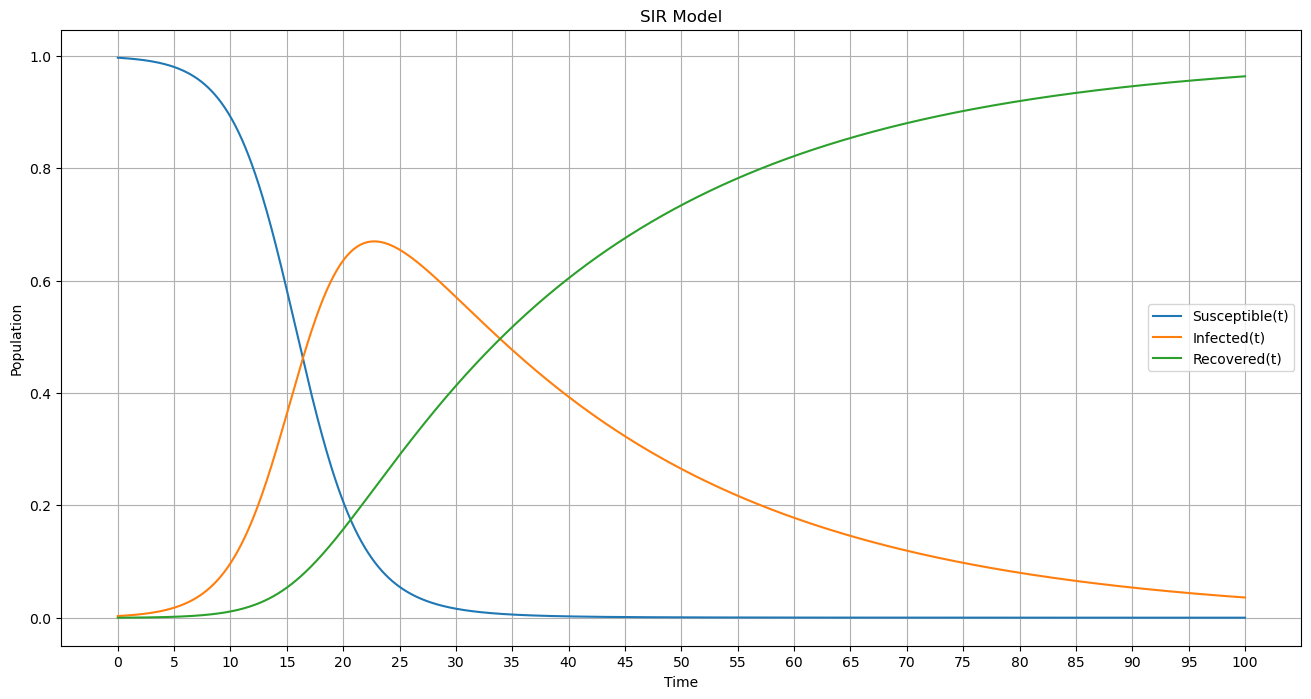
\includegraphics[scale=0.45]{images/img01}
		\caption{Зависимость $S, I, R$ от времени при начальных условиях $S(0) = 997$, $I(0) = 3$, $R(0) = 0$
			интенсивности инфицирования $\beta = 0.4$ и интенсивности выздоровления $\gamma = 0.04$}
		\label{fig:img01}
	\end{figure}
	
	Мы видим, что количество восприимчивых со времен уменьшается, число переболевших увеличивается, а число зараженных достигает своего пика приблизительно на 23 день, а затем их количество уменьшается. В реальной жизни происходит такой же процесс. Это говорит о том, что количество переболевших, то есть имеющих иммунитет, быстро растет, соответственно число зараженных уменьшается. Это и есть коллективный иммунитет, когда население становится невосприимчивым к штампу
	вируса. 
	
	Стоит учитывать, что данная модель является
	базовой: здесь мы не рассматривали вероятность вакцинации населения, то есть коллективный иммунитет был приобретен естественным путем; к тому же мы можем заметить, что по модели SIR в число выздоровевших попадают люди, которые погибли от данного заболевания. Это является одним их минусов
	данного моделирования. Базовая модель SIR служит отправной точкой для разработки более сложных моделей, включающих такие характеристики, как демографические группы с различными рисками
	для здоровья, естественные показатели
	рождаемости и смертности и влияние стохастичности (случайности). Как раз влияние стохастичности мы рассмотрим в следующем пункте. 
	
	\subsection{Рандомизация базовой модели SIR}
	В детерминированной математической модели (2) предполагается, что все
	параметры математической модели известны: число новых заразившихся пропорционально числу зараженных и восприимчивых к заражению индивидуумов.
	При этом при одинаковых начальных условиях и одинаковых параметрах математической модели всегда будет получено одинаковое решение. Однако в действительности эпидемический процесс подвержен случайным флуктуациям. Новые случаи заражения фактически происходят в условиях неопределенности, которую
	детерминированная модель учесть не может. Таким образом, становится
	актуальным применение стохастических математических моделей, учитывающих
	случайную составляющую.
	
	Одним из способов моделирования стохастических процессов является
	использование марковских цепей, то есть последовательности случайных
	событий, характеризующейся тем свойством, что при известном настоящем
	будущее независимо от прошлого. Цепи Маркова часто называют системами
	без последствия или системами с отсутствием памяти. 
	
	Другим способом моделирования является применение стохастических
	дифференциальных уравнений. Стохастическое дифференциальное уравнение -- дифференциальное уравнение, в котором один или несколько членов
	представляют собой стохастический процесс, приводящий к решению, которое
	само по себе является стохастическим процессом.
	
	Произведем обобщение базовой SIR-модели, добавив к ней рандомизацию. То есть мы приведем обыкновенные дифференциальные уравнения (6) к стохастическим дифференциальным уравнениям путем добавления к каждому уравнению, или же скорости изменения, белого шума $\epsilon_i(t) \sim \mathcal N (0,1)$, $i=1,2,3$. Тогда получим систему стохастических дифференциальных уравнений 
	\begin{equation}
		\left\{ 
		\begin{gathered} 
			\begin{aligned}
				\dfrac {\d s(t)}{\d t} &= -\beta \cdot s(t) \cdot i(t) + \epsilon_1(t),\\
				\dfrac{\d i(t)}{\d t} &= \beta \cdot s(t)\cdot i(t) - \gamma\cdot i(t) + \epsilon_2(t),\\
				\dfrac{\d r(t)}{\d t} &= \gamma\cdot i(t) + \epsilon_3(t). 
			\end{aligned}
		\end{gathered} 
		\right.		
	\end{equation}
	Причем нам нужно, чтобы для этой системы стохастических дифференциальных уравнений выполнялось соотношение (7), а значит \begin{equation}
		\epsilon_1(t) + \epsilon_2(t) + \epsilon_3(t) = 0.
	\end{equation}
	Чтобы это было верно, зададим случайный шум следующим образом.
	По сути единственные значения, в которых может появиться шум -- это интенсивности инфицирования $\beta$ и выздоровления $\gamma$. Поэтому
	пусть \begin{eqnarray}
		&\epsilon_1(t) = -\sigma_1 \cdot s(t)\cdot i(t) \cdot dW(t),\\
		&\epsilon_1(t) = \sigma_1 \cdot s(t)\cdot i(t) \cdot dW(t) - \sigma_2(t)\cdot i(t)\cdot dW(t),\\
		&\epsilon_3(t) = \sigma_2 \cdot i(t) \cdot dW(t),
	\end{eqnarray}
	где $dW (t)$ – производная стохастического винеровского процесса, введенная
	в систему дифференциальных уравнений исходя из предположения, что внешние
	случайные возмущения представляют собой белый шум; $\sigma_1, \sigma_2$ -- это константы, описывающие интенсивность стохастического окружения для процессов инфицирования
	и выздоровления соответственно. 
	
	Подставим данные выражения в систему уравнений (16) и получим систему стохастических дифференциальных уравнений с наложенными на нее условиями\begin{equation}
		\left\{ 
		\begin{gathered} 
			\begin{aligned}
				\dfrac {\d s(t)}{\d t} &= -\beta \cdot s(t) \cdot i(t) -\sigma_1 \cdot s(t)\cdot i(t) \cdot dW(t),\\
				\dfrac{\d i(t)}{\d t} &= \beta \cdot s(t)\cdot i(t) - \gamma\cdot i(t) + \sigma_1 \cdot s(t)\cdot i(t) \cdot dW(t) - \sigma_2(t)\cdot i(t)\cdot dW(t),\\
				\dfrac{\d r(t)}{\d t} &= \gamma\cdot i(t) + \sigma_2 \cdot i(t) \cdot dW(t). 
			\end{aligned}
		\end{gathered} 
		\right.		
	\end{equation}
	\begin{equation}
		s(t)\Big|_{t=t_0} = s_0,\quad i(t)\Big|_{t=t_0} = i_0,\quad r(t)\Big|_{t=t_0} = 0,
	\end{equation}
	Что при вынесении общих множителей как раз и показывает добавление стохастичности к интенсивностям:
	\begin{equation}
		\left\{ 
		\begin{gathered} 
			\begin{aligned}
				\dfrac {\d s(t)}{\d t} &= -\Big(\beta +\sigma_1 \cdot dW(t)\Big)\cdot s(t)\cdot i(t) ,\\
				\dfrac{\d i(t)}{\d t} &= \Big(\beta +\sigma_1 \cdot dW(t)\Big) \cdot s(t)\cdot i(t) - \Big(\gamma + \sigma_2d W(t)\Big)\cdot i(t),\\
				\dfrac{\d r(t)}{\d t} &= \Big(\gamma + \sigma_2d W(t)\Big)\cdot i(t). 
			\end{aligned}
		\end{gathered} 
		\right.		
	\end{equation}
	При этом стохастический винеровский процесс (броуновское движение)
	$W (t)$ является гауссовским процессом с независимыми приращениями, нулевым
	математическим ожиданием и дисперсией $\textbf D \{W(t)\} = t$. Следует также отметить, что при $\sigma_1 = 0$; $\sigma_2 = 0$
	стохастическая модель (21) становится детерминированной (6). 
	
	Существует несколько численных методов для решения стохастических дифференциальных уравнений, в том числе
	метод Эйлера-Маруямы, метод Мильштейна, стохастический метод Хойна, стохастический
	метод Рунге-Кутта. 
	
	Возьмем простейший численный метод для решения системы стохастических дифференциальных уравнений -- метод Эйлера-Маруямы. Для построенной стохастической SIR-модели схема Эйлера-Маруямы выглядит следующим образом
	\begin{equation}
		\left\{ 
		\begin{gathered} 
			\begin{aligned}
				\Delta t &= t_{j+1} - t_j,\\
				W_{j+1} &= \epsilon_j(0, \sqrt{\Delta t}),\\
				\Delta W_{j+1} &= W_{j+1} - W_j,\\
				s_{j+1} &= s_j - \beta s_j i_j \Delta t - \sigma_1 s_j i_j \Delta W_{j+1},\\
				i_{j+1} &= i_j + (\beta s_j i_j - \gamma i_j)\Delta t + \sigma_1 s_j i_j \Delta W_{j+1} - \sigma_2 i_j \Delta W_{j+1},\\
				r_{j+1} &= r_j + \gamma i_j\Delta t + \sigma_2 i_j \Delta W_{j+1},
			\end{aligned}
		\end{gathered} 
		\right.\quad t=0, 1,\ldots, T,		
	\end{equation}
	где $\epsilon_j(0, \sqrt{\Delta t})$ --- это некоторое случайное число из нормального распределения со средним $0$ и дисперсией $\sqrt{\Delta t}$.
	При этом для компьютерной реализации метода также необходимо задать некоторые исходные условия: $s_0$, $i_0$, $r_0$, $W_0 = \epsilon_0(0, \sqrt{\Delta t})$, $\Delta W_0  = W_0$.
	
	В качестве примера рассмотрим все ту же модель распространения заболеваний. Временной отрезок, который мы будем рассматривать, $T = 100$ дней. Мы проводим эксперимент над группой из $N=1000$ индивидуумов, среди которых $S(t_0) = 997$ индивидуумов восприимчивы к инфицированию, а $I(t_0) = 3$ индивидуума инфицировано. Также зададим среднюю интенсивность заражения $\beta = 0.4$ и среднюю интенсивность выздоровления $\gamma = 0.04$, то есть предположительно болезнь в среднем длится $D = 25$ дней.
	
	Результат численного решения такой задачи приложен на Рис.4. (см. Приложение 2)
	\begin{figure}[h]
		\centering
		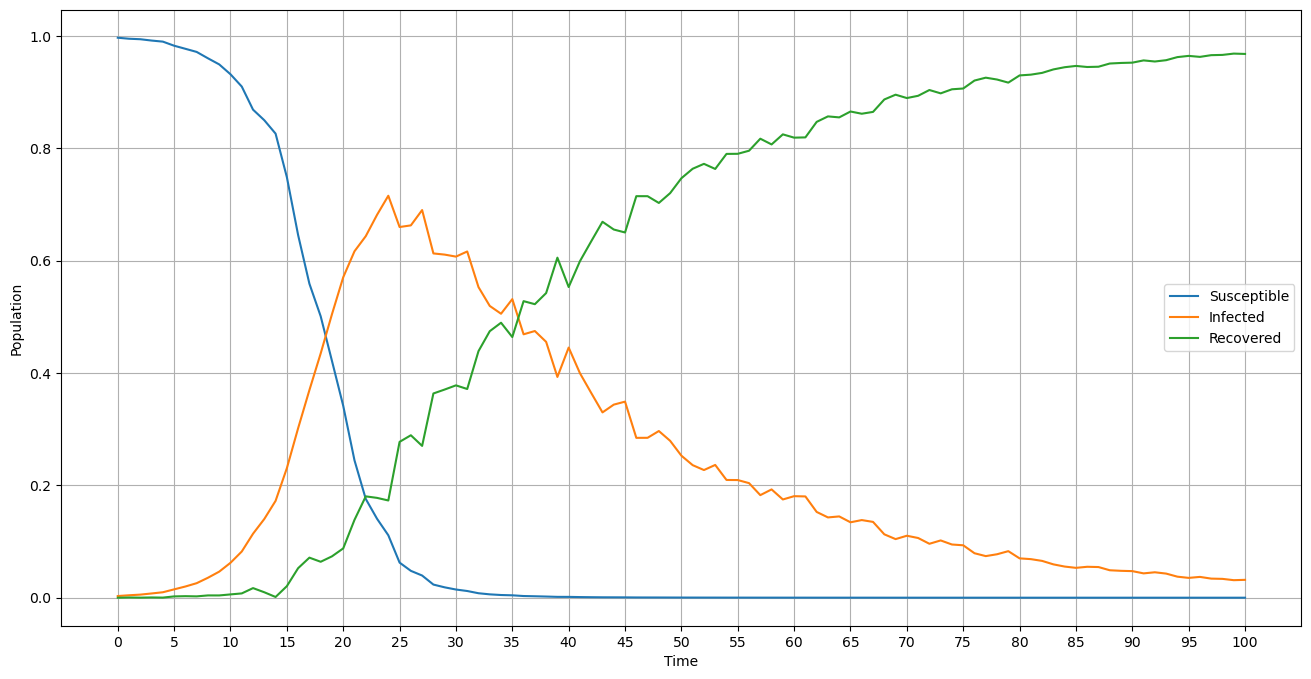
\includegraphics[scale=0.45]{images/img04}
		\caption{Зависимость $S, I, R$ от времени при начальных условиях $S(0) = 997$, $I(0) = 3$, $R(0) = 0$
			интенсивности инфицирования $\beta = 0.4$ и интенсивности выздоровления $\gamma = 0.04$ при $\sigma_1 = 0.1$, $\sigma_2 = 0.05$}
		\label{fig:img04}
	\end{figure}
	
	То есть, как можно увидеть, наши исходные кривые стали иметь гораздо больше изгибов, на что в принципе и повлиял элемент случайности, который мы добавили в модель. То есть для каждого индивидуума, вообще говоря, интенсивность инфицирования и выздоровления различна.
	\newpage
	\section*{ЗАКЛЮЧЕНИЕ}\addcontentsline{toc}{section}{ЗАКЛЮЧЕНИЕ}
	В данной работе рассмотрена SIR-модель описания динамики развития инфекционного процесса. Модель SIR (susceptible, infectious, recovered), описывающая распространение эпидемии, является базовой при применении подходов математического моделирования, так как в простейшем варианте включает в себя основные фазы эпидемии и в то же время допускает их уточнение с помощью корректирующих членов в уравнениях, а также добавления в систему исходных разрешающих уравнений новых уравнений. Модель SIR удобно использовать для модификации детерминированного подхода в вероятностный, поскольку она учитывает тот факт, что эпидемиологические процессы протекают в условиях наличия неполной информации и погрешностей наблюдения. 
	
	В случае модели SIR с рандомизацией было добавлено влияние случайности на классическую модель, что приближает нас к реальному отображению процесса распространения заболеваний.
	
	В мире появляются новые возбудители
	болезней, которые могут привести к эпидемии, есть также множество инфекционных заболеваний, которые человечеству
	еще предстоит победить, но и наука не
	стоит на месте, развивается, появляются
	новые методы выявления и борьбы с инфекционными заболеваниями, здесь велика роль математики и математического
	моделирования. Данная тема является
	очень обширной и актуальной, особенно в
	контексте нашего времени.
	\newpage
	\section*{СПИСОК ИСТОЧНИКОВ}\addcontentsline{toc}{section}{СПИСОК ИСТОЧНИКОВ}
	\begin{enumerate}
		\item Statistical forecasting of the dynamics of epidemiological indicators for COVID-19 incidence in the Republic of Belarus / Yu. S. Kharin, V. A. Valoshka, O. V. Dernakova, V. I. Malugin, A. Yu. Kharin// Journal of the Belarusian State University. Mathematics and Informatics. - 2020. - № 3. - С. 36-50
		\item Methods of intellectual data analysis in COVID-19 research / O. V. Senko, A. V. Kuznetsova, E. M. Voronin, O. A. Kravtsova, L. R. Borisova, I. L. Kirilyuk, V. G. Akimkin// Journal of the Belarusian State University. Mathematics and Informatics. – 2022. – № 1. – С. 83-96
		\item Детерминированные и стохастические модели распространения инфекции и тестирование в изолированном контингенте/ Чигарев, А. В.,Журавков, М. А.,Чигарев, В. А.// Журнал Белорусского государственного университета. Математика. Информатика - 2021. - № 3. - С. 57-67
		\item Lazzizzera, I. (2021) An Analytic Approximate Solution of the SIR Model. Applied Mathematics, 12, 58-73
		\item Contribution to the Mathematical Theory of Epidemics. Proceedings of the Royal Socoety A/ Kermack, W.O. and McKendrick, A.G. (1927) //115, 700-721.
	\end{enumerate}
	\newpage
	\section*{ПРИЛОЖЕНИЕ}\addcontentsline{toc}{section}{ПРИЛОЖЕНИЕ}
	\subsection*{Приложение 1}\addcontentsline{toc}{subsection}{Приложение 1}
	\begin{python}
		import numpy as np
		import matplotlib.pyplot as plt
		from scipy.integrate import odeint
		
		beta = 0.4
		gamma = 0.04
		
		def model(y, t):
		s, i, r = y
		dsdt = -beta * s * i
		didt = beta * s * i - gamma * i
		drdt = gamma * i
		return [dsdt, didt, drdt]
		
		t0 = 0
		t_end = 100
		t = np.linspace(t0, t_end, 1000) 
		
		s0 = 0.997
		i0 = 0.003
		r0 = 0.0
		
		y0 = [s0, i0, r0]
		sol = odeint(model, y0, t)
		
		s = sol[:, 0]
		i = sol[:, 1]
		r = sol[:, 2]
		
		plt.figure(figsize=(16, 8))
		plt.plot(t, s, label='Susceptible')
		plt.plot(t, i, label='Infected')
		plt.plot(t, r, label='Recovered')
		plt.xlabel('Time')
		plt.xticks(np.arange(min(t), max(t)+1, 5))
		plt.ylabel('Population')
		plt.title('SIR Model')
		plt.legend()
		plt.grid(True)
		plt.show()
	\end{python}
	
	\subsection*{Приложение 2}\addcontentsline{toc}{subsection}{Приложение 2}
	\begin{python}
		import numpy as np
		import matplotlib.pyplot as plt
		
		def euler_maruyama_sir_model(beta, gamma, S0, I0, R0, T, dt, sigma_1, sigma_2):
		N = int(T / dt)
		
		S = np.zeros(N+1)
		I = np.zeros(N+1)
		R = np.zeros(N+1)
		W = np.zeros(N+1)
		dW = np.zeros(N+1)
		
		S[0] = S0
		I[0] = I0
		R[0] = R0
		W[0] = np.random.normal(loc=0, scale=np.sqrt(dt))
		dW[0] = W[0]
		
		for j in range(N):
		W[j+1] = np.random.normal(loc=0, scale=np.sqrt(dt))
		dW[j+1] = W[j+1] - W[j]
		
		S[j+1] = S[j] - beta * S[j] * I[j] * dt - sigma_1 * S[j] * I[j] * dW[j+1]
		I[j+1] = I[j] + (beta * S[j] * I[j] - gamma * I[j]) * dt + sigma_1 * S[j] * I[j] * dW[j+1] - sigma_2 * I[j] * dW[j+1]
		R[j+1] = R[j] + gamma * I[j] * dt + sigma_2 * I[j] * dW[j+1]
		
		return S, I, R
		
		beta = 0.4
		gamma = 0.04
		S0 = 0.997
		I0 = 0.003
		R0 = 0
		T = 100
		dt = 1
		sigma_1 = 0.1
		sigma_2 = 0.05
		
		S, I, R = euler_maruyama_sir_model(beta, 
		gamma, 
		S0, 
		I0, 
		R0, 
		T, 
		dt, 
		sigma_1,
		sigma_2)
		
		t = np.arange(0, T+dt, dt)
		plt.figure(figsize=(16, 8))
		plt.plot(t, S, label='Susceptible')
		plt.plot(t, I, label='Infected')
		plt.plot(t, R, label='Recovered')
		plt.xlabel('Time')
		plt.ylabel('Population')
		plt.legend()
		plt.xticks(np.arange(min(t), max(t)+1, 5))
		plt.grid(True)
		plt.show()
	\end{python}
\end{document}